
\chapter[Decision trees (1 of 2)]{\huge\selectfont{Decision
trees for classification (1 of 2)}}
\label{ch:decisionTrees1}

So far our classification picture has been very general. We haven't said
anything about how our classifier might actually \textit{work}; we've just said
that given values for each of the features, it will render a prediction about
what the label will be.

\index{decision tree}
\index{random forest}

In chapters~\ref{ch:decisionTrees1} and \ref{ch:decisionTrees2}, we'll study
one particular algorithm for classification in machine learning: the
\textbf{decision tree} algorithm. Not only does it make a good introductory
technique because of its intuitive appeal, and not only can it classify pretty
well in its own right, but it also serves as the basis for a more
sophisticated, state-of-the-art classification method called ``\textbf{random
forest}'' which we'll explore in Volume II of this series.

\section{A working example}

\index{catalog} \index{videogames}

Here's a (fictitious) domain problem that
we'll use to demonstrate the principles in this chapter and the next. Say we
own a videogame business, and we want to send full-color product catalogs to
unsuspecting college students, so that they will buy our games and keep us in
business (while meanwhile failing out of school due to playing games all the
time).

Now full-color catalogs are expensive to print and ship, so we want to be smart
about this. We definitely don't want to send a bunch of catalogs to students
who aren't likely buyers; that would run our business into the ground. Instead,
we'd like to identify the subset of students who probably gamers, and send
catalogs to only \textit{those} students.

Suppose that through nefarious means, we have acquired the following data set:

\begin{Verbatim}[fontsize=\small,samepage=true,frame=single,framesep=3mm,xleftmargin=2.8cm,xrightmargin=2.7cm]
    Major  Age Gender   VG
 0   PSYC   22      F   No
 1   MATH   20      F   No
 2   PSYC   19      F   No
 3   CPSC   20      M  Yes
 4   MATH   18      M  Yes
 5   CPSC   20      F   No
 6   CPSC   19      O   No
 7   CPSC   17      M  Yes
 8   PSYC   18      F   No
 9   CPSC   20      F   No
 10  MATH   18      F   No
 11  CPSC   22      F  Yes
 12  MATH   21      M   No
 13  CPSC   23      M  Yes
 14  PSYC   17      M  Yes
 15  CPSC   18      F   No
 16  PSYC   19      F  Yes
\end{Verbatim}

\index{Psychology}
\index{Mathematics}
\index{Computer Science}

Each row represents one college student, with three features. The first is
their major -- \texttt{PSYC} (Psychology), \texttt{MATH} (Mathematics), or
\texttt{CPSC} (Computer Science). (For simplicity, we'll say these are the only
three possibilities, since your author happens to like them the best.) The
second is their age (numeric), and the third is their gender: male, female, or
other. The last column is our target: \textit{whether or not this student is a
videogamer.} Glance over this \texttt{DataFrame} for a moment.

\subsection{Eyeing the prior}

\index{value\_counts@\texttt{.value\_counts()} method (Pandas)}

As you remember from section~\ref{prior}, before we even think about features,
we might take a minute to just look at the target variable itself. We ask
ourselves ``given no other information about a student, what would be our gut
feel about their videogame status?'' Our pal the \texttt{.value\_counts()}
method is perfect to compute this:

\begin{Verbatim}[fontsize=\small,samepage=true,frame=single,framesep=3mm]
print(students.VG.value_counts())
\end{Verbatim}
\vspace{-.4in}

\begin{Verbatim}[fontsize=\small,samepage=true,frame=leftline,framesep=5mm,framerule=1mm]
N    10
Y     7
Name: VG, dtype: int64
\end{Verbatim}

So if we're smart, we'd guess ``no'' for such mysterious persons, but we could
only expect to be right about $\frac{10}{17}^\textrm{ths}$, or 59\%, of the
time. Not great, although better than a coin flip.

\smallskip
\subsection{Sticking with categorical features}

\index{categorical variable}

Now it turns out that decision trees work best with all categorical features,
not a mix of categorical and numeric. So for now, we're going to simply
classify each of our students into three buckets: ``\texttt{young}'' (18 or
younger), ``\texttt{middle}'' (19-21), and ``\texttt{old}''
(22+).\footnote{\index{Swift@Swift, Taylor} Believe it or not, a time will come in
your life when 22 years of age does not remotely seem ``old.'' For undergrads,
though, I can see why 22 would seem on the grey side, the Taylor Swift song
notwithstanding.} For the moment, don't ask why we chose three age categories
instead of two or four, and don't ask why we chose those particular split
points. We just did. More on that later.

% TODO: this is probably where to put the bin-into-categorical stuff.

\smallskip
Our training data now looks like this:
\label{vgDataSet}

\begin{Verbatim}[fontsize=\small,samepage=true,frame=single,framesep=3mm,xleftmargin=2.3cm,xrightmargin=2.5cm]
    Major     Age Gender   VG
 0   PSYC     old      F   No
 1   MATH  middle      F   No
 2   PSYC  middle      F   No
 3   CPSC  middle      M  Yes
 4   MATH   young      M  Yes
 5   CPSC  middle      F   No
 6   CPSC  middle      O   No
 7   CPSC   young      M  Yes
 8   PSYC   young      F   No
 9   CPSC  middle      F   No
 10  MATH   young      F   No
 11  CPSC     old      F  Yes
 12  MATH  middle      M   No
 13  CPSC     old      M  Yes
 14  PSYC   young      M  Yes
 15  CPSC   young      F   No
 16  PSYC  middle      F  Yes
\end{Verbatim}

and we're now officially ready to consider decision trees.

\section{Decision Trees}

\index{decision tree}
\index{root (of a decision tree)}

First, let's get our head around what a decision tree \textit{is}. Our
inaugural example is shown in Figure~\ref{fig:decisionTree}. The first thing
you'll notice is that it has a branching structure that branches...down. I'm
not sure why Data Scientists draw trees growing \textit{down} while the rest of
the world (including trees themselves: look outside if you don't believe me)
has them growing \textit{up}, but this is the convention so we'll just deal
with it. To make it even more comical, the oval at the top of the tree is
called the \textbf{root} of the tree. Really.

\begin{figure}[ht]
\centering
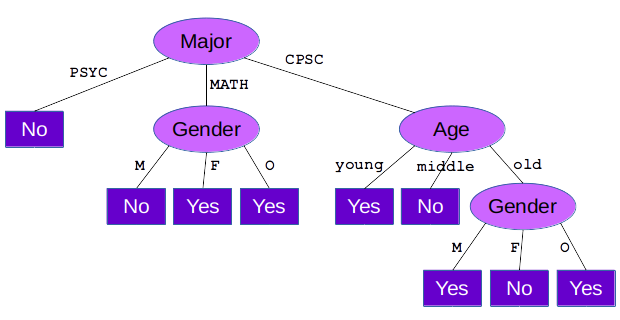
\includegraphics[width=0.9\textwidth]{decisionTree.png}
\caption{A decision tree (not a particularly good one, as it'll turn out) for
the videogame data set.}
\label{fig:decisionTree}
\end{figure}

\index{branch (of a decision tree)}
\index{leaf (of a decision tree)}
\index{node (of a decision tree)}

Continuing full bore with the botany analogy, the lines connecting the various
shapes are, as you might suspect, called \textbf{branches}, and the darker
rectangles are called \textbf{leaves}. One non-botanic bit of lingo is the name
for the other ovals: they're called \textbf{nodes}.

\subsection{Classifying with a decision tree}

Okay. Now what does a decision tree ``mean?'' Geekily-put, it's the pictorial
codification of an algorithm for classification. Not so geekily, it's a map
that tells your classifier what rules to follow as it forms its prediction for
an example data point.

You simply start at the root, considering feature values at each node, and
following the matching branch down the tree. When you reach a leaf, the
prediction you give is written on the leaf node. It's that simple.

\begin{itemize}

\label{decisionTreeExamples}
\item[\leftpointright] First example: suppose we have a 24-year-old male
Psychology major. We want to know whether he's likely to play videogames. The
decision tree in Figure~\ref{fig:decisionTree} tells us to first consider his
\textsf{Major}, since that's the root. Now because this guy's major is
\texttt{PSYC}, we take the left branch and are immediately done: we've already
reached a leaf. Our prediction for this guy will be \texttt{No}, he probably
doesn't play videogames.

\item[\leftpointright] Second example: we have an 18-year-old Math major who
doesn't identify with either of the binary genders. Starting again at the root,
we now follow the middle branch for \texttt{MATH}. Now, we look at the person's
\textsf{Gender}. Since it is \texttt{O}, we follow the right branch, and give a
prediction of \texttt{Yes}: we predict they \textit{do} play videogames.

\item[\leftpointright] Third example: we now have a 22-year-old female Computer
Science major. Do we think she would play videogames? The root tells us to look
at her \textsf{Major} first, which means we go right; then we look at her
\textsf{Age}, and since she's positively ancient we go right again; and
finally, her \textsf{Gender} tells us to predict \texttt{No}, she's probably
not a gamer.

\end{itemize}

Most students find this process very straightforward. In the next chapter,
we'll look at two key questions: first, how to turn a diagram like
Figure~\ref{fig:decisionTree} into Python code? And second, what's the best way
to make a \textit{good} tree -- \textit{i.e.}, one that makes as many
successful predictions as possible? 

